\documentclass[12pt,a4paper]{report}
\usepackage[utf8]{vietnam}
\usepackage{amsmath}
\usepackage{amsfonts}
\usepackage{amssymb}
\usepackage{makeidx}
\usepackage{graphicx}
\usepackage{fancybox}
\usepackage[left=3.50cm, right=2.00cm, top=3.50cm, bottom=3.00cm]{geometry}
\renewcommand{\baselinestretch}{1.5}
\usepackage{scrextend}
\changefontsizes{13pt}
\usepackage{fancyhdr}
\pagestyle{fancy}
\lhead{\textit{Đồ án tốt nghiệp đại học}}
\chead{}
\rhead{\textit{GVHD:PGS.TS Đỗ Đức Thuận}}
\lfoot{\textit{SVTH: Hoàng Thanh Lưu}}
\cfoot{\thepage}
\rfoot{\textit{Toán Tin K61}}
\renewcommand{\headrulewidth}{0.4pt}
\renewcommand{\footrulewidth}{0.4pt}
\begin{document}
	\thisfancypage{%đóng khung trang này
		\setlength{\fboxsep}{0pt}% 8pt là độ dày của đường viền
		\fbox}{} % phần nội dung sau là tương tự như đã làm
	\thispagestyle{empty}
	\begin{center}
		\vspace*{0cm}
		\fontsize{14}{12}
		\textbf{TRƯỜNG ĐẠI HỌC BÁCH KHOA HÀ NỘI}\\
		\textbf{VIỆN TOÁN ỨNG DỤNG VÀ TIN HỌC}\\
		\textbf{------ o0o ------}
	\end{center}
	\vspace*{0.4cm}
	\begin{figure}[h]
		\centering
		
\includegraphics[scale=.55]{./image/logo.png}
	\end{figure}
	\vspace*{0.4cm}
	\begin{center}
		\fontsize{20}{18}
		\textbf{ĐIỀU KHIỂN TỐI ƯU CHUYỂN ĐỘNG THẲNG CỦA TÊN LỬA}\\
		\vspace*{1.2cm}
		\fontsize{18}{16}
		\textbf{ĐỒ ÁN TỐT NGHIỆP ĐẠI HỌC}\\
		\fontsize{14}{16}
		\vspace*{0.4cm}
		\textit{Chuyên ngành:} \textbf{Toán Tin}
	\end{center}
	\vspace*{0.7cm}
	\begin{center}
		\fontsize{14}{16}
		\begin{tabular}{ll}
			
			\textbf{Giảng viên hướng dẫn:} & \textbf{PGS.TS ĐỖ ĐỨC THUẬN } \\ 
			\textbf{Sinh viên thực hiện:} & \textbf{HOÀNG THANH LƯU} \\ 
			\textbf{Lớp:}  & \textbf{TOÁN TIN K61} \\ 
		\end{tabular} \\
		\vspace*{1.6cm}
		\fontsize{14}{16}
		\textbf{Hà Nội - 12/2020}
	\end{center}
	\newpage
	\thispagestyle{empty}
	
	\chapter*{Lời nói đầu}
	\pagenumbering{arabic}
	\setcounter{page}{1}
	\textbf{Lý do chọn đề tài}\\\\
	Khi phải thiết kế, xây dựng bất kì một hệ thống điều khiển nào đó, các nhà thiết kế thường gặp phải bài toán thiết kế làm sao cho hệ thống đạt được chất lượng làm việc mong muốn như: tính ổn định, mức tiêu hao năng lượng thấp, tính bền vững cao...\\\\ Điều khiển tối ưu là một phần mở rộng của phép tính biến phân, là một phương pháp tối ưu hóa cho các lý thuyết điều khiển phát sinh.Điều khiển tối ưu có thể được xem như là một phương án điều khiển trong lý thuyết điều khiển tự dộng.\\\\
	\textbf{Đối tượng và phạm vi nghiên cứu} \\\\
	Đồ án đi sâu vào nghiên cứu cụ thể một số bài toán trong điều khiển tối ưu như:
	\begin{itemize}
		\item Bài toán liên quan đến điều khiển tối ưu cho các trạng thái cuối cùng có ràng buộc
		\item Cách chứng minh và giải ví dụ về bài toán
	\end{itemize}
	\textbf{Phương pháp nghiên cứu}
	\begin{itemize}
		\item Nghiên cứu lý thuyết: Phân tích các công trình được công bố ở lĩnh vực liên quan, thông qua bài giảng giáo án trên lớp
		\item Nghiên cứu thực tiển
		\item Lấy ý kiến chuyên gia: Tham khảo ý kiến của thầy giáo trực tiếp hướng dẫn.
	\end{itemize}
	Em xin gửi lời cảm ơn sâu sắc đến thầy Đỗ Đức Thuận đã giúp đỡ em hoàn thiện được đề tài !
	
	\chapter{Kiến thức cơ bản}
	
	\chapter{Điều khiển tối ưu chuyển động thẳng của tên lửa}
	
	Trong khuôn khổ đồ án này, chúng ta mô hình hóa bài toán tối đa hóa vận tốc của tên lửa chuyển động tịnh tiến bằng bài toán điều khiển tối ưu tuyến tính, trong đó điều khiển biểu diễn hành động của phi công trên tên lửa. Để giải quyết mô hình thu được, chúng ta áp dụng cả phương pháp phân tích và phương pháp số. Lời giải phân tích được tính bằng nguyên lý cực đại Pontryagin trong khi lời giải gần đúng của bài toán được giải quyết bằng phương pháp chụp cũng như hai kỹ thuật tùy biến: kỹ thuật sử dụng công thức Cauchy và kỹ thuật sử dụng công thức Euler. Để so sánh các phương pháp khác nhau, chúng ta sẽ phát triển một triển khai với MATLAB và trình bày một số kết quả mô phỏng.
	
	\section{Giới thiệu}
	Điều khiển tối ưu là một lĩnh vực rất quan trọng trong toán học ứng dụng. Thật vậy, nhiều bài toán thực tế có thể được mô hình hóa dưới dạng các bài toán điều khiển tối ưu. Lý thuyết điều khiển tối ưu được áp dụng thành công trong nhiều lĩnh vực như cơ khí, kỹ thuật điện, hóa học, sinh học, hàng không và vũ trụ, robot, nông nghiệp, v.v.\\Cách tiếp cận truyền thống để giải quyết các vấn đề điều khiển tối ưu là sử dụng nguyên lý cực đại Pontryagin. Nguyên tắc này, do L.S. Pontryagin đưa ra vào năm 1956, tổng quát hóa các phương trình Euler-Lagrange của phép tính các biến thể và đưa ra một điều kiện tối ưu cần thiết. Lý thuyết điều khiển cũng được áp dụng trong các ngành toán học khác nhau: điều khiển tối ưu các phương trình vi phân riêng, lý thuyết điều khiển ngẫu nhiên, lý thuyết trò chơi,... Bài toán điều khiển tối ưu có thể được giải quyết bằng nguyên lý cực đại Pontryagin, tuy nhiên khi bài toán khó, chúng ta phải sử dụng phương pháp số để tìm một giải pháp gần đúng.
	\\Trong đồ án này, chúng ta đưa ra một mô hình điều khiển tuyến tính tối ưu với thời gian cuối tự do để tối đa hóa vận tốc của tên lửa chuyển động theo chuyển động thẳng từ vị trí ban đầu đến vị trí cuối cùng. Để giải quyết mô hình thu được, chúng ta áp dụng cả phương pháp phân tích và phương pháp số. Giải pháp phân tích được tính toán bằng cách sử dụng nguyên lý cực đại Pontryagin, trong khi lời giải gần đúng của bài toán được tìm thấy bằng cách sử dụng phương pháp chụp và hai kỹ thuật tùy chỉnh: kỹ thuật tùy chỉnh Cauchy và một kỹ thuật tùy chỉnh Euler. Các vấn đề lập trình tuyến tính thu được được giải quyết một cách hiệu quả với một phương pháp điểm bên trong được thực hiện trong Matlab.
	\section{Mô hình hóa bài toán}
	Xét một tên lửa có khối lượng $m$ và vận tốc $v(t)$ tại thời điểm $t \in [0, T]$, chuyển động từ độ cao ban đầu $h(0)$ đến độ cao cuối cùng $h(T)$ với chuyển động thẳng nghiêng. Sử dụng các định luật vật lý cho các vật thể chuyển động thẳng nghiêng \textbf{[tl1, tl2]}, chúng ta thu được phương trình sau:
	$$\dfrac{d^2h}{dt^2}(t) = \dfrac{T_p(t)}{m} - g, t \in [0, T],$$
	trong đó $h(t)$ và $T_p(t)$ tương ứng là quãng đường đi được và lực đẩy của tên lửa tại thời điểm $t\in[0, T]$, $g$ là gia tốc trọng trường. Ta đặt $w(t) = \dfrac{T_p(t)}{m}$ và $\dfrac{dh}{dt}(t) = v(t)$. Do đó, chúng ta nhận được
	\begin{eqnarray}
		\begin{cases}
			\dfrac{dh}{dt}(t) = v(t), \\ \dfrac{dv}{dt}(t) = w(t) - g, t \in [0, T].
		\end{cases}
	\end{eqnarray}
	Nếu phi công không áp dụng bất kỳ lệnh nào trên tên lửa, thì lực đẩy $w(t)$ thỏa mãn phương trình sau:
	\begin{equation}
		\dot{w}(t) = \alpha w(t), t \in [0, T].
	\end{equation} trong đó $\alpha$ > 0 là nghịch đảo của thời gian đáp ứng của động cơ tên lửa đối với ứng dụng thí điểm. Để điều khiển chuyển động của tên lửa, phi công tác dụng một lực $u(t), t \in [0, T]$. Phương trình vi phân thông thường (2.2) trở thành: \begin{equation}
	\dot{w}(t) = \alpha[w(t) - u(t)], t \in [0, T].
\end{equation}
Do đó, mục tiêu là để vận tốc của tên lửa chuyển động từ điểm ban đầu $h(0) = h_0$ đến độ cao $h_1$ cho trước là cực đại. Điều này dẫn chúng ta đến việc giải quyết vấn đề điều khiển tối ưu sau:
\begin{eqnarray}
	\begin{cases}
		\text{Maximize } J(u, T) = v(T), \\ \dot{h}(t) = v(t), \\ \dot{v}(t) = w(t) - g, \\ \dot{w}(t) = \alpha[w(t) - u(t)],\\ h(0) = h_0, v(0) = 0, w(0) = g, \\ h(T) = h_1, |u(t)| \leq 1, t \in [0, T], T \text{ tự do.}
	\end{cases}
\end{eqnarray}
Bài toán này được viết dưới dạng ma trận sau: 
\begin{eqnarray}
	\begin{cases}
		\text{Maximize } J(u, T) = c'x(T), \\ \dot{x}(t) = Ax(t) + Bu(t) + r, \\ x(0) = x_0, Q'x(T) = h_1, |u(t)|\leq 1, t \in [0, T], T \text{ tự do.}
	\end{cases}
\end{eqnarray} trong đó 
$$x(t) = \begin{pmatrix}
	h(t) \\ v(t) \\ w(t)
\end{pmatrix}, x(0) = \begin{pmatrix}
0 \\ 0 \\ g
\end{pmatrix}, A = \begin{pmatrix}
0&1&0 \\ 0&0&1 \\ 0&0& \alpha
\end{pmatrix}$$\\
$$B = \begin{pmatrix}
	0\\0\\-\alpha
\end{pmatrix}, r = \begin{pmatrix}
0\\-\alpha\\0
\end{pmatrix},$$\\
$$Q'=(1,0,0) \text{ và } c'=(0,1,0).$$ trong đó ký hiệu $A'$ ký hiệu chuyển vị của ma trận $A$, $A$ là ma trận bất kỳ. \\Ma trận Kalman được cho bởi:  $$K = (B, AB, A^2B) = \begin{pmatrix}
	0&0&-\alpha\\0&-\alpha&-\alpha^2\\-\alpha&-\alpha^2&-\alpha^3
\end{pmatrix}, det(K) = \alpha^3 \neq 0.$$ Hạng của ma trận $K$ là hạng $(K) = 3$, do đó hệ thống (2.5) có thể điều khiển được.
	\section{Tối thiểu hóa thời gian}
	Bây giờ chúng ta tính giá trị của thời gian cuối cùng $T$, giá trị này sẽ được sử dụng trong bài toán (2.4), bằng cách giải bài toán tối thiểu thời gian sau:
	\begin{eqnarray}
		\begin{cases}
			\text{Minimize } J(u, T) = \int_{0}^{T}dt, \\ \dot{h}(t) = v(t), \\ \dot{v}(t) = w(t) - g, \\ \dot{w}(t) = \alpha[w(t) - u(t)], \\h(0) = h_0, v(0) = 0, w(0) = g, \\ |u(t)| \leq 1, h(T) = h_1, t\in [0, T].
		\end{cases}
	\end{eqnarray}
	Để giải quyết bài toán (2.6), chúng ta sử dụng nguyên lý cực đại Pontryagin. Biểu thị bằng $p(t) = (p_h(t), p_v(t), p_w(t))$ là vectơ phụ liên quan đến bài toán (2.6), có hàm Hamilton được cho như sau: \begin{eqnarray}
		H(t, x(t), p(t), p^0, u(t)) = p_h(t)v(t) + p_v(t)[w(t) - g] \nonumber\\ + \alpha p_w(t)[w(t) - u(t)] + p^0
	\end{eqnarray}
	Vì chúng ta cực đại hóa hàm Halminton, chúng ta đặt $p_0 = -1$.\\ Các vectơ liền kề là nghiệm của hệ tương ứng với các phương trình Euler-Lagrange sau:
	\begin{eqnarray}
		\begin{cases}
			\dot{p}_h(t) = 0, \\ \dot{p}_v(t) = -p_h(t), \\ \dot{p}_w(t) = -p_v(t) - \alpha p_w(t), t \in [0, T].
		\end{cases}
	\end{eqnarray}
	Từ hệ thức (2.8), ta suy ra
	\begin{eqnarray}
		\begin{cases}
			p_h(t) = \lambda_1, \\ p_v(t) = -\lambda_1t + \lambda_2, \\ p_w(t) = \dfrac{1}{\alpha^2}(\alpha^2\lambda_3e^{-\alpha t} + \alpha\lambda_1t - \lambda_1 - \alpha\lambda_2), \\ \lambda_i \in \mathbb{R}, i = 1,2,3,
		\end{cases}
	\end{eqnarray} với \begin{eqnarray}
	p_h(0) = \lambda_1, p_v(0) = \lambda_2, p_w(0) = \dfrac{1}{\alpha^2}(-\lambda_1-\alpha\lambda_2 + \alpha^2\lambda_3), \\ H(0, x(0), p(0), u(0)) = \alpha p_w(0)[g - u(0)] - 1.
\end{eqnarray} Hệ động lực là tự điều khiển, do đó hàm Hamilton là hằng số với mọi $t \in [0, T]$. Do đó, chúng ta sẽ có \begin{equation}
H(0, x(0), p(0), u(0)) = H(T, x(T), p(T), u(T)).
\end{equation} Vì thời điểm cuối cùng $T$ là tự do, theo điều kiện của tính ngang giá, chúng ta nhận được: \begin{equation}
H(T, x(T), p(T), u(T)) = 0.
\end{equation}
Từ (2.12) và (2.13), ta thu được $$H(0, x(0), p(0), u(0)) = \alpha p_w(0)[g-u(0)] - 1 = 0.$$ Vì vậy \begin{eqnarray}
	p_w(0) = \dfrac{1}{\alpha[g-u(0)]} > 0.
\end{eqnarray}
Giá trị cực đại của hàm Halminton được cho bởi \begin{eqnarray}
	H(t, x^*(t), p^*(t), u^*(t)) &=& \max_{-1 \leq u(t) \leq 1}H(t, x(t), p(t), u(t)) \nonumber\\ &=&p_h(t)v(t) + p_v(t)[w(t)-g] \nonumber\\&+& \alpha p_w(t)w(t) - 1 + \alpha \max_{-1 \leq u(t) \leq 1}[-p_w(t)u(t)]. \nonumber
\end{eqnarray} Do đó, điều khiển tối đa hóa Hamilton là: \begin{equation}
u^*(t) = -\text{sign}(p_w(t))
\end{equation}
Từ (2.14) và (2.15) chúng ta có $u^*(0) = -1.$ \\\\Nếu cố định thời gian đáp ứng của động cơ là $0.7s$, chúng ta tìm thấy $\alpha = 1.42$ và sử dụng các dữ liệu sau để giải quyết bài toán (2.6): $h_0=0m, h_1 = 600m, g = 9.80665m.s^{-2}$. Mục tiêu là xác định thời gian tối thiểu, tối ưu của bài toán. Bằng cách sử dụng phương pháp chụp, chúng ta thu được kết quả như Hình 2.1.
\begin{figure} [h]
	\centering
	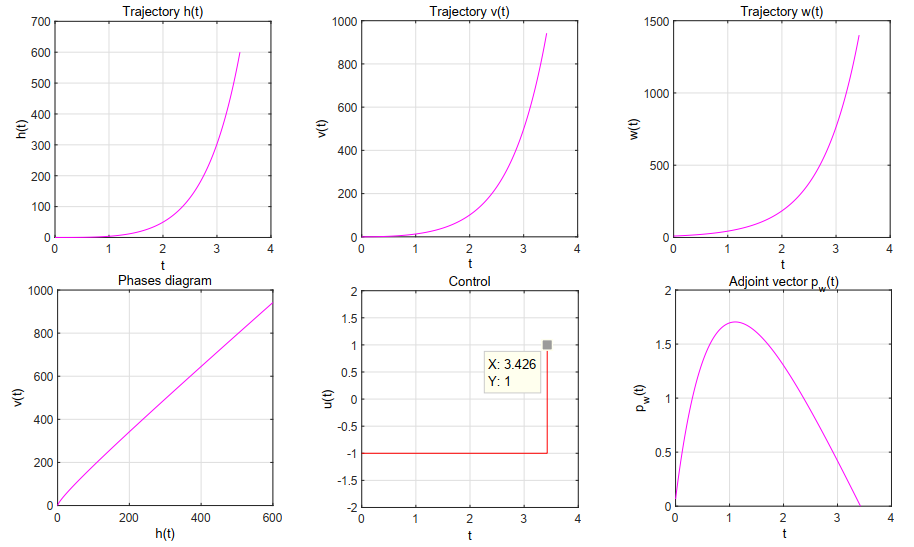
\includegraphics[scale=.6]{./image/hinh1.png}
	\caption{Kết quả của bài toán tối ưu thời gian}
\end{figure}
\\Phương pháp chụp dựa trên nguyên lý cực đại Pontryagin. Nó bao gồm việc tìm ra điểm 0 của chức năng chụp liên quan đến vấn đề thời gian tối thiểu. Đây là một phương pháp nhanh, độ chính xác cao, không yêu cầu giả định về cấu trúc điều khiển. Phương pháp chụp bao gồm ba bước chính:
\begin{itemize}
	\item \textbf{Bước 1:}
	Hình thành một bài toán giá trị biên bằng cách sử dụng các phương trình mô hình và các phương trình vectơ liền kề cũng như các điều kiện ngang.
	\item \textbf{Bước 2:}
	Xác định hàm chụp.
	\item \textbf{Bước 3:}
	Giải hệ phương trình phi tuyến.
\end{itemize}
Từ đồ thị Hình 2.1, ta suy ra $T_{\min} = 3.43s$. Biết thời gian tối thiểu này, thời gian cuối cùng của chúng ta luôn được chọn lớn hơn một chút so với $T_{\min}$. Vì vậy, chúng ta chọn $T = 3.5s$.
	\section{Bài toán vận tốc cực đại của tên lửa}
	Trong phần này, coi như thời gian cuối cùng, thời gian $T$ tìm thấy trong phần trước, tức là $T = 3.5$ giây. Đầu tiên chúng ta giải quyết vấn đề (2.4) bằng phân tích; sau đó chúng ta tiến hành phân giải số bằng 3 phương pháp: phương pháp chụp, phương pháp tùy chỉnh Cauchy và phương pháp tùy chỉnh Euler. \\
	Để giải bài toán (2.4), trước hết chúng ta áp dụng nguyên lý cực đại Pontryagin. Hàm Hamilton của
	bài toán (2.4) với $t \in [0, T]$ là
	\begin{equation}
		H(t, x(t), p(t), u(t)) = p_h(t)v(t) + p_v(t)[w(t)-g] + \alpha p_w(t)[w(t)-u(t)]
	\end{equation} Các vectơ liền kề là nghiệm của hệ sau:
\begin{eqnarray}
	\begin{cases}
		\dot{p}_h(t) = 0, \\ \dot{p}_v(t) = -p_h(t), \\ \dot{p}_w(t) = -p_v(t) - \alpha p_w(t), t \in [0, T]
	\end{cases}
\end{eqnarray}
Từ hệ thức (2.17), ta suy ra rằng
\begin{eqnarray}
	\begin{cases}
		p_h(t) = \lambda_1, \\ p_v(t) = -\lambda_1t+\lambda_2, \\ p_w(t) = \dfrac{1}{\alpha^2}(\alpha^2\lambda_3e^{-\alpha t} + \alpha\lambda_1t - \lambda_1 - \alpha\lambda_2), \\ \lambda_i \in \mathbb{R}, i = 1,2,3
	\end{cases}
\end{eqnarray} với \begin{eqnarray}
p_h(0) = \lambda_1, p_v(0) = \lambda_2, p_w(0) = \dfrac{1}{\alpha^2}(\lambda_1-\alpha\lambda_2+\alpha^2\lambda_3)
\end{eqnarray}
Cực đại hàm Halminton được cho bởi \begin{eqnarray}
	H(t, x^*(t), p^*(t), u^*(t)) &=& \max_{-1 \leq u(t) \leq 1}H(t, x(t), p(t), u(t)) \nonumber \\ &=& p_h(t)v(t) + p_v(t)[w(t)-g]\nonumber \\ &&+\alpha p_w(t)w(t) \nonumber \\&& + \alpha \max_{-1 \leq u(t) \leq 1}[-p_w(t)u(t)]. \nonumber
\end{eqnarray}
Điều khiển tối ưu Hamilton là \begin{equation}
	u^*(t) = -\text{sign}(p_w(t))
\end{equation}
Vectơ $x(T)$ phải thỏa mãn ràng buộc
$$h_1-Q'x(T)=0$$ Vì thời điểm cuối cùng $T$ là cố định trong bài toán (2.4), chúng ta nhận được các điều kiện chuyển đổi sau:
\begin{eqnarray}
	-p_h(T) - \dfrac{\partial g(x(T))}{\partial h(T)} + \dfrac{\partial(h_1 - Q'x(T))}{\partial h(T)}b = 0, \\
	-p_v(T) - \dfrac{\partial g(x(T))}{\partial v(T)} + \dfrac{\partial(h_1 - Q'x(T))}{\partial v(T)}b = 0, \\ -p_w(T) - \dfrac{\partial g(x(T))}{\partial w(T)} + \dfrac{\partial(h_1 - Q'x(T))}{\partial w(T)}b = 0,
\end{eqnarray} với $g(x(T)) = -v(T)$ và $b \in \mathbb{R}$. \\Từ đó, chúng ta có được các điều kiện biên sau: \begin{equation}
p_h(T) = -b, p_v(T) = 1, p_w(T) = 0
\end{equation}
Bằng cách sử dụng các điều kiện biên (2.24) và các mối quan hệ (2.18), chúng ta nhận được:
\begin{eqnarray}
	\begin{cases}
		p_h(t) = -b, \\ p_v(t) = b(t-T) + 1,  \\ p_w(t) = \dfrac{1}{\alpha^2}((a-b)(e^{-\alpha(t-T)} - 1) - \alpha b(t-T)),  \\ t\in[0, T].
	\end{cases}
\end{eqnarray}
	\subsection{Giải pháp phân tích}
	Vì điều khiển tối ưu bằng dấu đối nghịch của vectơ liền kề $p_w(t)$, nên thời gian giao hoán là
	được cho bởi nghiệm nguyên của phương trình $p_w(t) = 0$. Vì $A$ là ma trận bậc 3 và tất cả các giá trị riêng của $A$ là thực nên bài toán có nhiều nhất một thời gian giao hoán $t_c < T$ \\Để chọn chiến lược tối ưu, hãy xem xét các chiến lược khả thi sau:
	\begin{itemize}
		\item \textbf{Chiến lược 1} $u(t) = 1, \forall t \in [0, T]$; 
		\item \textbf{Chiến lược 2} $u(t) = -1, \forall t \in [0, T]$; \item
		\textbf{Chiến lược 3} $u(t) = 1$ với $t \in [0, t_c]$, sau đó $u(t) = -1$ với $t \in [t_c, T]$;
		\item \textbf{Chiến lược 4} $u(t) = -1$ với $t \in [0, t_c]$, sau đó $u(t) = 1$ với $t \in [t_c, T].$
	\end{itemize}

\subsubsection{Chiến lược 1}
Chúng ta có $\dot{w}(t) = \alpha[w(t) - 1]$, nghĩa là: 
\begin{eqnarray}
	\begin{cases}
		w(t) = c_1e^{\alpha t} + 1, \\ v(t) = \dfrac{c_1}{\alpha}e^{\alpha t} + (1-g)t + c_2, \\ h(t) = \dfrac{c_1}{\alpha^2}e^{\alpha t} + \dfrac{(1-g)}{2}t^2+c_2t+c_3, c_1, c_2, c_3 \in \mathbb{R}
	\end{cases}
\end{eqnarray} 
Sử dụng các điều kiện ban đầu, chúng ta thu được:
\begin{eqnarray}
	\begin{cases}
		w(t) = (g-1)e^{1.42t}+1, \\ v(t) = (g-1)\bigg(\dfrac{1}{1.42}e^{1.42t}-t-\dfrac{1}{1.42}\bigg) \\ h(t) = (g-1)\bigg(\dfrac{1}{1.42^2}e^{1.42t}-\dfrac{1}{2}t^2-\dfrac{1}{1.42}t - \dfrac{1}{1.42^2}\bigg).
	\end{cases}
\end{eqnarray}
 Với $t = T$, chúng ta sẽ có $h(T) = 549.0243 < 600.$ Do đó \textbf{Chiến lược 1} là không khả thi
 \subsubsection{Chiến lược 2} Chúng ta có $\dot{w(t)} = \alpha[w(t) + 1]$, nghĩa là: 
 \begin{eqnarray}
 	\begin{cases}
 		w(t) = d_1e^{\alpha t} - 1, \\ v(t) = \dfrac{d_1}{\alpha}e^{\alpha t} - (1+g)t + d_2, \\ h(t) = \dfrac{d_1}{\alpha^2}e^{\alpha t} - \dfrac{(1+g)}{2}t^2+d_2t+d_3, d_1, d_2, d_3 \in \mathbb{R}
 	\end{cases}
 \end{eqnarray} 
Sử dụng các điều kiện ban đầu, chúng ta thu được: 
\begin{eqnarray}
	\begin{cases}
		w(t) = (g+1)e^{1.42t}+1, \\ v(t) = (g+1)\bigg(\dfrac{1}{1.42}e^{1.42t}-t-\dfrac{1}{1.42}\bigg) \\ h(t) = (g+1)\bigg(\dfrac{1}{1.42^2}e^{1.42t}-\dfrac{1}{2}t^2-\dfrac{1}{1.42}t - \dfrac{1}{1.42^2}\bigg).
	\end{cases}
\end{eqnarray}
Với $t = T$, chúng ta sẽ có $h(T) = 673.7083 > 600$, vì vậy \textbf{Chiến lược 2} là không khả thi.

\subsubsection{Chiến lược 3}
Phương trình của tập quỹ đạo đầu tiên, khi $u(t) = 1, t \in [0, t_c]$ là: 
\begin{eqnarray}
	\begin{cases}
		w(t) = (g-1)e^{1.42t}+1, \\ v(t) = (g-1)\bigg(\dfrac{1}{1.42}e^{1.42t}-t-\dfrac{1}{1.42}\bigg) \\ h(t) = (g-1)\bigg(\dfrac{1}{1.42^2}e^{1.42t}-\dfrac{1}{2}t^2-\dfrac{1}{1.42}t - \dfrac{1}{1.42^2}\bigg).
	\end{cases}
\end{eqnarray}
Phương trình của tập quũ đạo thứ hai, khi $u(t) = -1, t\in [t_c, T]$ được cho bởi: 
\begin{eqnarray}
	\begin{cases}
		w(t) = \beta_1 e^{1.42t} + 1, \\ v(t) = \dfrac{\beta_1}{1.42}e^{1.42t} - (g+1)t+\beta_2, \\ h(t) = \dfrac{\beta_1}{1.42^2}e^{1.42t} - \dfrac{(g+1)}{2}t^2 + \beta_2t + \beta_3, \text{ }  \beta_1, \beta_2, \beta_3 \in \mathbb{R}.
	\end{cases}
\end{eqnarray}
Tại giao điểm của hai tập hợp, ta thu được: \begin{eqnarray}
	\beta_1 = (g-1) + 2e^{-1.42t_c}, \text{ } \beta_2 = 2t_c - \dfrac{(g+1)}{1.42}, \text{ } \beta_3 = -t_c^2 + \dfrac{2}{1.42}t_c - \dfrac{(g+1)}{1.42^2} \nonumber
\end{eqnarray}
Tính $t_c$ sao cho $h(T) = 600m$. Điều kiện cuối cùng này dẫn đến phương trình sau: \begin{equation}
	142.86e^{-1.42t_c} - t_c^2 + 8.41t_c - 69.15 = 0.
\end{equation}
Nghiệm số của phương trình cuối cùng này là $t_c = 0.557s.$ \\ Bằng cách thay các giá trị của $\beta_1$ và $\beta_2$ vào phương trình thứ hai của hệ (2.31), chúng ta thu được $$J(u, T) = v(T) = 940.8949\text{ }m.s^{-1}$$

\subsubsection{Chiến lược 4}
Phương trình của tập quỹ đạo đầu tiên, khi $u(t) = -1, t\in[0, t_c]$ là: \begin{eqnarray}
	\begin{cases}
		w(t) = (g+1)e^{1.42t}-1, \\ v(t) = (g+1)\bigg(\dfrac{1}{1.42}e^{1.42t}-t-\dfrac{1}{1.42}\bigg) \\ h(t) = (g+1)\bigg(\dfrac{1}{1.42^2}e^{1.42t}-\dfrac{1}{2}t^2-\dfrac{1}{1.42}t - \dfrac{1}{1.42^2}\bigg).
	\end{cases}
\end{eqnarray}
Phương trình của tập quỹ đạo thứ hai, khi $u(t) = 1, t \in[t_c, T]$ được cho bởi: \begin{eqnarray}
	\begin{cases}
		w(t) = \gamma_1e^{\alpha t} + 1, \\ v(t) = \dfrac{\gamma_1}{\alpha}e^{\alpha t} + (1-g)t + \gamma_2, \\ h(t) = \dfrac{\gamma_1}{\alpha^2}e^{\alpha t} + \dfrac{(1-g)}{2}t^2 + \gamma_2t + \gamma_3, \text{ } \gamma_1, \gamma_2, \gamma_3 \in \mathbb{R}. 
	\end{cases}
\end{eqnarray}
Tại giao điểm của hai tập hợp, ta thu được: $$\gamma_1 = (g+1) - 2e^{-1.42t_c}, \text{ } \gamma_2 = -2t_c - \dfrac{(g-1)}{1.42}, \text{ } \gamma_3=t_c^2 - \dfrac{2}{1.42}t_c-\dfrac{(g-1)}{1.42^2}.$$ Tính toán $t_c$ sao cho $h(T) = 600m$. Điều kiện cuối cùng này tạo ra phương trình sau:
\begin{equation}
	142.8555e^{-1.42t_c} + t_c^2 + 8.4085t_c + 91.8798 = 0.
\end{equation} Nghiệm số của phương trình cuối cùng này là $t_c = 0.331s$\\Theo hệ thức (2.34), giá trị mục tiêu của bài toán (2.4) bằng: $$J(u, T) = v(T) = 931.6531 \text
{ } m.s^{-1}.$$ Lưu ý rằng giá trị mục tiêu được đưa ra bởi \textbf{Chiến lược 3} cao hơn giá trị được tìm thấy trong \textbf{Chiến lược 4}, thuộc loại bang-bang. Các kết quả lý thuyết được vẽ trong Hình 2.2 và Hình 2.3.
\begin{figure}[h]
	\centering
	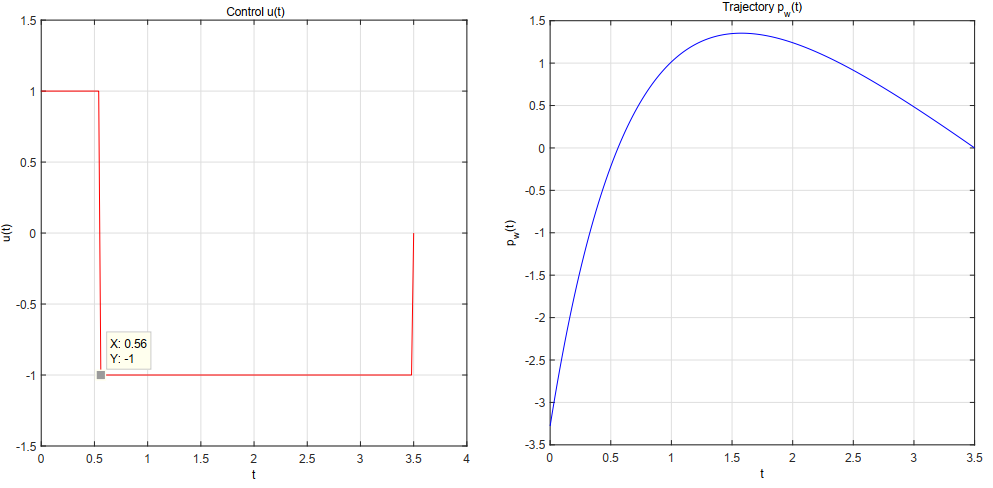
\includegraphics[scale=.6]{./image/hinh2.png}
	\caption{$t \to u(t)$ và $t \to p_w(t)$}
\end{figure}
Do đó, chúng ta đã xác định được quỹ đạo tối ưu đạt cực đại $v(T)$ và thỏa mãn điều kiện biên $h(T) = 600m$, được cho bởi
\begin{eqnarray}
u^*(t) =	\begin{cases}
		1, & t \in [0, 0.55];\\ -1, & t\in[0.55, 3.5];
	\end{cases}
\end{eqnarray} và $$J(u^*, T) = v^*(T) = 940.8949 \text{ } m.s^{-1}.$$

\begin{figure}[h]
	\centering
	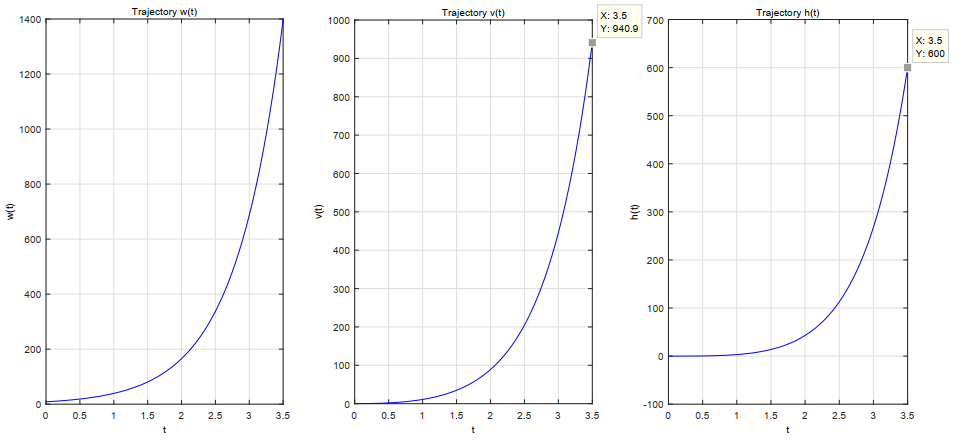
\includegraphics[scale=.6]{./image/hinh3.png}
	\caption{Quỹ đạo tối ưu $t \to h(t), t\to v(t)$ và $t\to w(t)$}
\end{figure}
	\subsection{Độ phân giải số theo phương pháp chụp}
	
	\subsection{Độ phân giải số theo phương pháp tùy chỉnh Cauchy}
	
	\subsection{Độ phân giải số bằng phương pháp tùy biến Euler}
	
	\subsection{So sánh số}
	
	
	\chapter{Kết luận}
	
	
\end{document}